% !TEX root =  ../gesamtkonzept.tex
\subsection{Architektur}

% TODO: hyperref auskommentiert, weil dazu ja nix existiert. -> integration in bestehende system könnte man eventuell erwähnen, wenn man das Backend von wo anders aus auch ansteuern wollen würde unso, man muss ja net unser frontend nutzen.
Das neue System setzt, wie \citeauthor{MS-Fielding.} empfiehlt, auf das Client-Server-Modell. Dabei soll ein mehrfacher und voneinander unabhängiger Zugriff sowie die Entwicklung von Erweiterungen oder die Integration in bereits bestehende Systeme ermöglicht werden.
%, womit Anforderung \hyperref[Anf:A1]{A1}, die Umsetzung des Systems als Webanwendung, abgedeckt werden soll.
Dabei stellt der Server, wie in Abbildung \ref{img:einkaufBPMN} zu erkennen, eine \ac{API} für den Client zur Verfügung, um auf die Geschäftslogik und somit alle Ressourcen zugreifen zu können.
Der Client ist somit lediglich für die Darstellung verantwortlich und übernimmt nur geringfügige Überprüfungen der Eingaben des Nutzers, sodass bei absehbar falschen Anfragen der Server nicht ausgelastet wird.
Zur Darstellung stellt der Client dabei die Visualisierungsmethoden zur Verfügung und arbeitet die von der Schnittstelle erhaltenen Daten auf.

\begin{figure}[h]
  \centering
  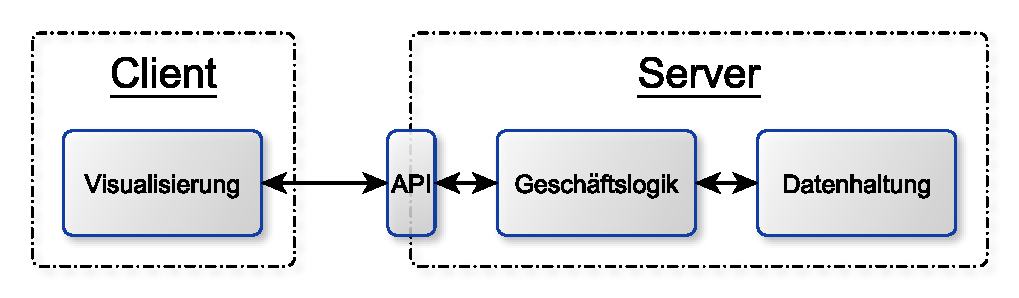
\includegraphics[width=0.75\textwidth]{img/konzeption/gesamtkonzept/Architektur.pdf}
  \captionsetup{format=hang,justification=raggedright,singlelinecheck=false}
  \caption[Architekturmodell]{Architekturmodell. \\Quelle: Eigene Darstellung.}
  \label{img:einkaufBPMN}
\end{figure}

Grundlegend ist deshalb die Architektur dem \ac{MVC}-Konzept nachempfunden, da der Server das Model durch die vorhandene Datenbank und die darin vorhandenen Relationen darstellt und die View des Konzepts durch den Client repräsentiert wird.
Der Controller wird dabei zu einem Teil durch die Geschäftslogik im Server und der damit verbundenen \ac{API} repräsentiert, ist jedoch ebenso im Client durch eine Sammlung und Aufarbeitung der Daten sowie einer geringfügigen Überprüfungen der Nutzereingaben vorhanden.\autocite{rf-leff2001web}
